\documentclass[fleqn]{article}
\usepackage{amsmath}
\usepackage[dvips]{graphicx}
\bibliographystyle{plain}
%__________________________________
\begin{document}

\section*{\center Exploding Container}
\subsection*{\underline{Problem Description}}

In this simulation, a two-dimensional slice of a steel container that
is filled with PBX-9501 has been ``preheated" to above the ignition temperature
of the explosive.  At t=0, the explosive begins to burn, and the resulting
product gas pressurizes the container which expands to the point of rupture.

\subsection*{\underline{Simulation Specifics}}
\begin{description} 
\item [Component used:] \hfill mpmice
\item [Input file name:] \hfill ExplodeContainer.ups
\item [Command used to run input file:]\hfill sus ExplodeContainer.ups

\item [Simulation Domain:]\hfill    0.09 x 0.09 x 0.002 m

\item [Cell Spacing:]\hfill \\ 
.001 x .001 x .002 m (Level 0)

\item [Example Runtimes:] \hfill \\
 5 hours   (1 processor, 3.0 GHz Xeon)\\
 The run time can be reduced to less than one hour by halving the number
 of cells in the x and y direction.

\item [Physical time simulated:] \hfill 0.12 milliseconds

\item [Associate scirun network:] \hfill ExplodeContainer.srn

\end{description}

\section*{\underline{Results}}

Figure~\ref{figexpcont} shows the container and the explosive as
represented by particles which are colored by mass.  A cutting plane
depicts the pressure field.  Note that some dark blue particles have
found their way through the container wall, which seems bad.  However,
a check of the colormap reveals that the mass of those particles is
vanishingly small, approximately machine zero, at which point they
become a bit hard to control.

\begin{figure}[b]
  \center
%  \scalebox{0.2}{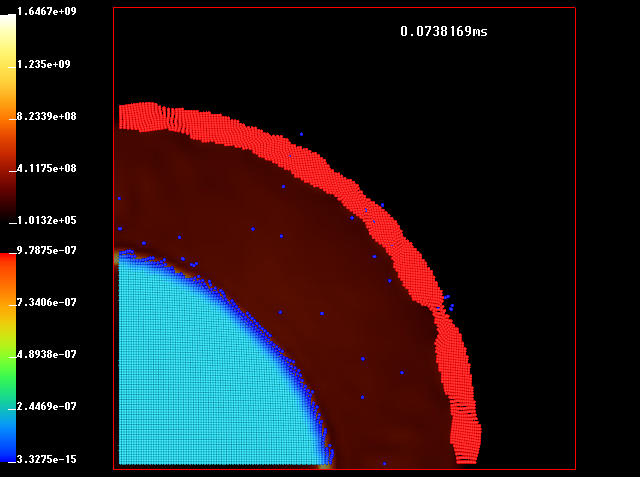
\includegraphics{ExplodeContainer.png}}
  \caption{Steel container filled with burning PBX-9501.}
  \label{figexpcont}
\end{figure}

\end{document}
